\documentclass[xcolor=dvipsnames,12pt,a4paper,oneside]{book}

%%%%%%%%%%%%%%%%%%%%%%%%%%%%%%%%%%%%%%%%%%%%%%%%%%%%%%%%%%%%%%%%%%%%%%%
%%%%%% Package-Sammlung %%%%%%%%%%%%%%%%%%%%%%%%%%%%%%%%%%%%%%%%%%%%%%%
%%%%%%%%%%%%%%%%%%%%%%%%%%%%%%%%%%%%%%%%%%%%%%%%%%%%%%%%%%%%%%%%%%%%%%%

\usepackage[utf8]{inputenc}
\usepackage[ngerman]{babel}
\usepackage{amsmath}
\usepackage{amsfonts}
\usepackage{amssymb}
\usepackage{graphicx}
\usepackage{footnote}
\usepackage{float}
\usepackage[labelfont=bf]{caption}
\usepackage{textcomp}
\usepackage{hyperref}
\usepackage[numbers]{natbib}
\usepackage{verbatim}
\usepackage{url}
\usepackage{pifont}
\usepackage{listings}
\usepackage{color}
\usepackage{microtype}
\usepackage{pdfpages}
\usepackage{acronym}
\usepackage{nomencl}
\usepackage{multirow}
\usepackage{makecell}
\usepackage{imakeidx}
\usepackage{setspace}
\usepackage{todonotes}
\usepackage{fontenc}
\newcommand{\Anhang}[1]{\textit{\appendixname{}~\ref{#1}: (\nameref{#1})}}
\newcommand{\Kapitel}[1]{\textit{Kapitel~\ref{#1} (\nameref{#1})}}
\newcommand{\Tabelle}[1]{\textit{Tabelle~\ref{#1} (\nameref{#1})}}
\newcommand{\Listing}[1]{\textit{Listing~\ref{#1} (\nameref{#1})}}
\newcommand{\Abbildung}[1]{\textit{Abbildung~\ref{#1} (\nameref{#1})}}
\newcommand{\Code}[1]{\texttt{#1}}
\newcommand{\Vgl}[1]{\cite{#1}}

\newcommand{\ua}{u.~a. }
\newcommand{\zB}{z.~B. }
\newcommand{\dasheisst}{d.~h. }
\newcommand{\bspw}{bspw. }
\newcommand{\bzw}{bzw. }

% Orphan- und Widow-Zeilen vermeiden
\widowpenalty10000
\clubpenalty10000

%%%%%%%%%%%%%%%%%%%%%%%%%%%%%%%%%%%%%%%%%%%%%%%%%%%%%%%%%%%%
%%%%%% Code-Eigenschaften %%%%%%%%%%%%%%%%%%%%%%%%%%%%%%%%%%
%%%%%%%%%%%%%%%%%%%%%%%%%%%%%%%%%%%%%%%%%%%%%%%%%%%%%%%%%%%%

\definecolor{mygreen}{rgb}{0,0.6,0}
\definecolor{mygray}{rgb}{0.5,0.5,0.5}
\definecolor{mymauve}{rgb}{0.58,0,0.82}

\lstset{ % Code-Optionen für Pseudocode
  backgroundcolor=\color{white},
  basicstyle=\footnotesize,
  breakatwhitespace=false,
  breaklines=true,
  captionpos=b,
  commentstyle=\color{mygreen},
  deletekeywords={...},
  escapeinside={\%*}{*)},
  extendedchars=true,
  frame=single,
  keepspaces=true,
  keywordstyle=\color{blue},
  language=Octave,
  otherkeywords={*,...},
  numbers=left,
  numbersep=5pt,
  numberstyle=\tiny\color{mygray},
  rulecolor=\color{black},
  showspaces=false,
  showstringspaces=false,
  showtabs=false,
  stepnumber=1,
  stringstyle=\color{mymauve},
  tabsize=2,
  title=\lstname
}


% Titelblatt
\setcounter{secnumdepth}{5}
\usepackage[left=2cm,right=2cm,top=2cm,bottom=2cm]{geometry}
\author{Uni Oldenburg, Florian Trei und Jonas Hellmann}				   		
\date{\today}  								   		
\title{Dokumentation Team Chillow - InformatiCup 2021}


%%%%%%%%%%%%%%%%%%%%%%%%%%%%%%%%%%%%%%%%%%%%%%%%%%%%
%%%%%%%%% Titelseite %%%%%%%%%%%%%%%%%%%%%%%%%%%%%%%
%%%%%%%%%%%%%%%%%%%%%%%%%%%%%%%%%%%%%%%%%%%%%%%%%%%%

\setlength{\parindent}{0pt}
\begin{document}
\lstset{language=Python}

\begin{titlepage}
\pagestyle{empty}
\begin{center}


\begin{figure}[H]
\centering

\includegraphics[width=0.35\textwidth]{Logo.jpg}
\end{figure}

\bigskip \bigskip \noindent
\textsc{\textbf{\LARGE InformatiCup 2021:}} \par \bigskip \noindent
\textsc{\textbf{\LARGE Dokumentation}}


\par \bigskip \bigskip \bigskip \bigskip \bigskip \noindent
{\Large Team Chillow} \par \medskip \noindent
{\Large (Florian Trei, Jonas Hellmann)} \par \medskip \noindent




\par \bigskip \bigskip \bigskip \bigskip \bigskip \bigskip \noindent
\begin{center} \Large Wintersemester 2020/21 \end{center}


\par \bigskip \bigskip \bigskip \bigskip \bigskip \bigskip \noindent
\textsf{\textbf{Spiel-Implementierung:\\spe\_ed}} \par \noindent
\textsf{\textbf{}}\par
\bigskip


\bigskip\bigskip\bigskip\bigskip\bigskip\noindent
Stand:\par\noindent
\today


\end{center}
\end{titlepage}


%%%%%%%%%%%%%%%%%%%%%%%%%%%%%%%%%%%%%%%%%%%%%%%%%%%%%%%
%%%%%%%%% Verzeichnisse %%%%%%%%%%%%%%%%%%%%%%%%%%%%%%%
%%%%%%%%%%%%%%%%%%%%%%%%%%%%%%%%%%%%%%%%%%%%%%%%%%%%%%%

\pdfbookmark[1]{Inhaltsverzeichnis}{inhalt}
\tableofcontents
\clearpage

\addcontentsline{toc}{chapter}{Abbildungsverzeichnis}
\listoffigures
\clearpage

\addcontentsline{toc}{chapter}{Tabellenverzeichnis}
\listoftables
\clearpage

\addcontentsline{toc}{chapter}{Listing-Verzeichnis}
\lstlistoflistings
\clearpage

\addcontentsline{toc}{chapter}{Abkürzungsverzeichnis}
\newcommand{\abkvz}{Abkürzungsverzeichnis}
\renewcommand{\nomname}{\abkvz}
\chapter*{\abkvz}
\markboth{\abkvz}{\abkvz}
\begin{acronym}[WWWWW]

\acro{KI}{Künstliche Intelligenz}

\end{acronym}
\clearpage


%%%%%%%%%%%%%%%%%%%%%%%%%%%%%%%%%%%%%%%%%%%%%%%%%%%%%%%
%%%%%%%%% Import der einzelnen Inhalte %%%%%%%%%%%%%%%%
%%%%%%%%%%%%%%%%%%%%%%%%%%%%%%%%%%%%%%%%%%%%%%%%%%%%%%%

\onehalfspacing
\chapter{Einleitung}
\label{ch:einleitung}

In dieser Dokumentation wird der Lösungsentwurf vom Team Chillow der Universität Oldenburg für den InformatiCup 2021,
der von der Gesellschaft für Informatik organisiert wird, beschrieben.
Das Team besteht aus den Mitgliedern Florian Trei und Jonas Hellmann, die zum Zeitpunkt des Wettbewerbs im fünften
Semester in den Studiengängen B. Sc. Informatik \bzw B. Sc. Wirtschaftsinformatik eingeschrieben sind.
Das Repository mit dem Quellcode zu der hier beschriebenen Lösung ist unter folgendem Link abrufbar:
\url{https://github.com/jonashellmann/informaticup21-team-chillow} \\

Die Aufgabenstellung\footnote{Eine genauere Beschreibung lässt sich in folgendem PDF-Dokument finden:
\url{https://github.com/informatiCup/InformatiCup2021/blob/master/spe\_ed.pdf}} sieht eine Implementierung des Spiels
\texttt{spe\_ed} vor.
Hierbei steuern bis zu sechs Spieler rundenbasiert eine Figur, die besuchte Felder markiert und bei einer Kollision
mit einem bereits markiertem Feld oder beim Verlassen des Spielfelds verliert.
Ziel ist es, eine eigenständig spielende \ac{KI} zu programmieren, die möglichst viele Spiele gewinnt.
\chapter{Einstieg in das Projekt}
\label{ch:planung}

Bevor mit der Implementierung der \ac{KI} begonnen werden konnte, mussten zuerst noch einge andere Punkte geklärt
\bzw erledigt werden.
Diese ersten Schritte werden im folgenden erläutert.

\section{Auswahl der Programmiersprache}
\label{sec:auswahl-programmiersprache}

Zu Beginn war zu klären, mit welcher Programmiersprache dieser Lösungsvorschlag umgesetzt werden soll.
Die Wahl ist dabei schnell auf Python gefallen, obwohl beide Gruppenmitglieder hiermit noch keinerlei Erfahrung
aufweisen konnte.
Der Grund für diese Entscheidung liegt neben dem starken Interessen an dem Kennenlernen einer neuen Programmiersprache
auch an der bereits sehr hohen und immer noch steigenden Popularität der Programmiersprache und der damit verbundenen
zukünftigen Wichtigkeit. \Vgl{tiobe} \Vgl{pypl}
Hinzu kommt, dass wir vor Beginn der Implementierung anhand der Aufgabenstellung das Potenzial für den Einsatz von
Machine Learning gesehen haben und Python in diesem Bereich oft empfohlen wird. \Vgl{springboard} \Vgl{towardsscience}

\subsection{Einsatz von Poetry als Build-Tool}
\label{subsec:poetry}

% Vorteile eines Build-Tools und Poetry im Speziellen
% Verwaltung von Abhängigkeiten mit Poetry

\section{Erstellung eines lauffähigen Projekts}
\label{sec:erstellung-projekt}

\subsection{Entwicklung eines Dockerfile}
\label{subsec:dockerfile}

Nachdem die Nutzung von Python feststand, haben wir zum Start ein minimales Python-Skript erstellt, das lediglich die
an den Docker-Container übergebenen Parameter für die Server-URL und den API-Key ausgibt.
Zwar mussten bis hierhin noch keine Abhängigkeiten hinzugefügt werden, aber bei der Konzeption des Dockerfiles sollte
bereits die Installtion zusätzlicher Bibliotheken berücksichtigt werden.
Mit der Nutzung des Standard-Python-Containers von Docker Hub wird bereits ein vorgefertigter Container bereitgestellt,
in dem Python und Pip installiert ist.
Anschließend wird mittels Pip die Installation von Poetry durchgeführt.
Dieses Tool wiederum bietet die Möglichkeit, die verwalteten Abhängigkeiten in Form einer
\texttt{requirements.txt}-Datei zu exportieren, welche dann von Pip eingelesen werden kann, um die Bibliotheken zu
installieren.
Später sind noch Umgebungsvariablen zur Steuerung des Programm-Ablaufs hinzugekommen, sodass das Dockerfile
letztendlich wie in \Listing{lst:dockerfile} dargestellt aussieht.

\begin{minipage}{\linewidth}
\lstinputlisting[label=lst:dockerfile,language=Java,caption=Dockerfile zum Erstellen eines lauffähigen Containers]
{../Dockerfile}
\end{minipage}

\section{Nachstellung des Spiels}
\label{sec:nachstellung-spiel}

% Spiel nachprogrammiert, um selbst offline gegen die KIs spielen zu können
% Vorgriff auf spätere Kapitel: Zentrale Funktionalitäten konnten später wiederverwendet werden
\chapter{Lösungsansatz}
\label{ch:loesungsansatz}

% Implementierung mehrerer AIs
% Ggf. Vorgehen beschreiben, wie die beste KI ermittelt wurde -> statistische Vorgehensweise, Grafiken
% Probleme bei Erstellung eines Baums, da bei Vorausberechnung viele Kombinationen entstehen
% Probleme für Reinforcement Learning, da Testdaten schwierig zu generieren sind


\section{Selbstlernende KI mithilfe von Trainingsdaten}
\label{sec:selbstlernende-ki-trainingsdaten}

Zunächst haben wir uns die Frage gestellt, ob eine \ac{KI} mithilfe von Trainingsdaten lernen soll.
Dieser Ansatz bringt jedoch das Problem mit sich, gute Trainingsdatensätze besitzen zu müssen.
Bei einer maximalen Anzahl von sechs Spielern im Spiel \texttt{spe\_ed} und 5 unterschiedlichen möglichen Aktionen gibt
es sehr viele Möglichkeiten, wie ein Spiel verlaufen kann.
Dabei entsteht das Problem zu beurteilen, welche Spielsituationen und welche Spielverläufe als Trainingsdaten gut
geeignet sind, sodass die gesamte Komplexität des Spiels in unseren Trainingsdaten abgebildet wird.
Aufgrund dessen haben wir uns dafür entschieden, zunächst Lösungsansätze ohne eine selbstlernende \ac{KI}
auszuprobieren.
Diese Strategie hatte für uns den Vorteil, mithilfe einfacherer Lösungsansätze die Komplexität und auftretenden Probleme
im Spielverlauf besser kennen zu lernen. \todo{weitere technische Begründung hinzufügen}


\section{Lösungsansätze ohne selbstlernende KIs}
\label{sec:loesungsansatz-ohne-selbstlernende-kis}

Bei dem Ansatz, Strategien fest in Code zu implementieren, hatten wir mehrere unterschiedliche Ideen,
die nachfolgend beschrieben werden.
Ziel war es hierbei, Teilprobleme zu erkennen und zu lösen, mit der Intuition diese unterschiedlichen \ac{KI}s
kombinieren zu können.

\subsection{RandomAI}
\label{subsec:random-ai}

Die \Code{RandomAI} ist unsere erste lauffähige KI gewesen und unser Maß für die einfachste \ac{KI}.
Diese stellt zwar keinen wirklichen Lösungsansatz dar, diente jedoch als Einstieg und um erste Probleme zu erkennen.
Durch die \Code{RandomAI} ist uns das grundlegende Problem aufgefallen, dass sich die \ac{KI} selber tötet.
Folglich wird die Minimal- und Maximalgeschwindigkeit überschritten, das Spielfeld verlassen oder in vorhandene Spuren
gefahren, mit denen eine Kollision vermeidbar gewesen wäre.

\subsection{NotKillingItselfAI}
\label{subsec:notkillingitself-ai}

Aufgrund des beschriebenen Problemes der \Code{RandomAI} haben wir uns dafür entschieden, die \Code{NotKillingItselfAI}
zu implementieren.
Die \ac{KI} soll aus allen Aktionen eine zufällige Aktion auswählt, die sie nicht direkt verlieren lässt.
Dazu wird für jede mögliche Aktion die Spur berechnet, die entstehen würde und auf Kollisionen überprüft.
Aktionen die eine Kollision hervorrufen werden nicht ausgeführt.
Hierbei bleiben mögliche Aktionen der Gegenspieler zunächst unberücksichtigt.\\

Durch die Implementierung der \Code{NotKillingItselfAI} fiel auf, dass die \ac{KI} sich zwar nicht mehr im unmittelbar
folgenden Zug tötete, jedoch häufig in Sackgassen läuft.
Dieses Problem wird in der \Abbildung{fig:Sackgassen_Problem} verdeutlicht.

\begin{figure}[htb]
    \centering
    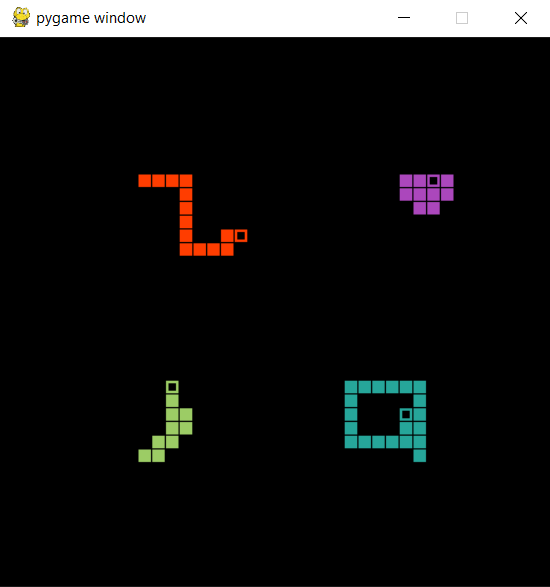
\includegraphics[width=0.6\textwidth]{Bilder/Sackgassen_Problem.png}
    \caption{\Code{NotKillingItselfAI} unten rechts in einer Sackgasse}
    \label{fig:Sackgassen_Problem}
\end{figure}

\subsection{PathfindingAI}
\label{subsec:pathfinding-ai}

Folglich der \Code{NotKillingItselfAI} haben wir einen Lösungsansatz gesucht, welcher das Betreten von Sackgassen
verhindert.
Genutzt wurde die Basis der \Code{NotKillingItselfAI}, sodass nur zwischen überlebenden Aktionen gewählt wird.
Um die Aktionen zu finden, die nicht in eine Sackgasse läuft, haben wir uns für einen Lösungsansatz zum Finden von
Pfaden entschieden.
Dazu wird eine konfigurierbare Anzahl Koordinaten generiert, auf denen sich bisher kein Spieler befindet.
Diese Koordinaten lassen sich sowohl gleichverteilt auf dem Spielfeld als auch zufällig generieren.
Anschließend wird für jede Aktion geprüft, zu wie vielen der Koordinaten, nach der Ausführung der Aktion noch ein
möglicher Pfad existiert. \todo{In einem Bild verdeutlichen warum das ein Bewertungskriterium darstellt}
Die Aktion, die die höchste Anzahl Koordinaten erreichen kann, führt mit höchster Wahrscheinlichkeit
nicht in eine Sackgasse und wird ausgewählt. \\

Bei diesem Lösungsansatz arbeiten wir lediglich mit der Wahrscheinlichkeit, dass wir nicht in eine Sackgasse laufen.
Dies liegt dem Problem zugrunde, dass wir die Implementierung eines Algorithmus zum tatsächtichen Erkennen von
Sackgassen oder abgesperrten Gebieten als schwieriger erachteten.

\subsection{SearchTreeAI}
\label{subsec:searchtree-ai}

Bei der \Code{PathfindingAI}, als auch der \Code{NotKillingItselfAI} gibt es weiterhin ein bestehendes
Problem.
Die \ac{KI} beachtet die möglichen Aktionen der Gegenspieler nicht.
Ziel der \Code{SearchTreeAI} ist es, dass die die \Code{NotKillingItselfAI}, falls möglich, auch nur Aktionen berechnet,
bei denen bereits alle möglichen gegnerischen Aktionen und dessen Auswirkungen berücksichtigt werden. \\

Unser Lösungsansatz für dieses Problem ist es, mithilfe eines Suchbaums alle möglichen gegnerischen
Aktions-Kombinationen zu prüfen und einen Teilbaum zu finden, bei dem vorausgesagt werden kann, dass
der eigene Spieler unabhängig der ausgewählten Aktion von allen anderen Spielern nicht im nächsten Zug stirbt.
Der Vorteil eines Suchbaums ist es, dass wir diesem eine
beliebige Tiefe mitgeben können, um entsprechend der Tiefe viele zukünftige Züge vor zu berechnen.
\todo{Besser ausformulieren, Problem der Komplexität benennen und Beispielskizze}

\chapter{Implementierung}
\label{ch:implementierung}

Den Einstieg in das Programm stellt die Datei \Code{main.py} dar.
Hier wird entschieden, ob ein Online- oder Offline-Spiel wie schon in den vorherigen Kapiteln beschrieben gestartet
werden soll.
Die Implementierungen dieser beiden Spielvarianten sollen in diesem Kapitel beschrieben werden, wobei der Fokus auf
die Online-Verbindung gerichtet ist, da es sich hierbei um die Umsetzung der eigentlichen Aufgabenstellung handelt.

\section{Modellierung des Spiels}
\label{sec:modellierung}

Um eine Grundlage zu haben, auf der die Implmentierung aufgebaut werden konnte, wurde als die Modellierung des Spiels
vorgenommen.
Dazu haben wir geschaut, welche Informationen benötigt und vom Server bereitgestellt werden und wie man diese dann
nach einem objektorientierten Ansatz abbilden kann.

Das Ergebnis der Modellierung ist in \Abbildung{fig:klassendiagramm-modell} zu sehen.
Das \Code{Game} hat Zugriff zum einen auf die eigenen Eigenschaften, kennt aber auch alle \Code{Player}, die an diesem
Spiel teilnehmen.
Zudem besteht ein \Code{Game} aus einem zweidimensionalen Array aus \Code{Cells}, die das Spielfeld repräsentieren.
In einer \Code{Cell} können sich dann kein, ein oder nach einer Kollision auch mehrere Spieler befinden.

\begin{figure}[htb]
\centering
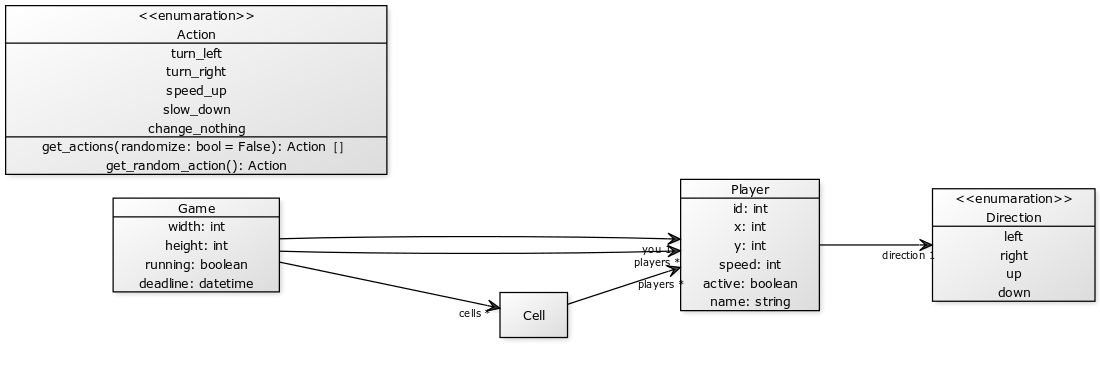
\includegraphics[width=\textwidth]{Bilder/Klassendiagramm_Modellierung.png}
\caption{UML-Klassendiagramm des Modells}
\label{fig:klassendiagramm-modell}
\end{figure}

Da ein Spieler in eine bestimmte Anzahl an Richtungen gedreht sein kann, wird diese Ausrichtung über die Enumeration
\Code{Direction} abgebildet.
Ebenso ist die Auswahl der möglichen Aktionen begrenzt, sodass diese in der Enumeration \Code{Action} festgelegt
worden sind.

\section{Implementierung des Online-Spiels}
\label{sec:online-implementierung}

Um eine Verbindung zu dem \Code{spe\_ed}-Server aufbauen zu können, müssen die URL und ein gültiger API-Key vor dem
Start der Anwendung als Umgebungsvariablen gesetzt worden sein.
Diese Websocket-URL wird entsprechend modifiziert auch als Endpunkt zur Abfrage der Server-Zeit verwendet, auf deren
Nutzung nachfolgend noch eingegangen wird.

Die zum Start des Spiels öffentlich bereitgestellte Methode \Code{play()} ist in \Listing{lst:online-play} dargestellt.
Diese ist sehr simpel und ruft lediglich die private Methode \Code{\_\_play()} auf.
Hierbei handelt es sich um eine asychrone Methode, wie schon in der Methoden-Signatur deutlich wird.
Es wird mittels der Bibliothek \Code{asyncio} sichergestellt, dass diese asynchrone Methode vollständig verarbeitet
wurde, bevor der Kontrollfluss im Programm weiterläuft.
Sobald dies der Fall ist, ist das Spielende eingetreten und die Oberfläche wird deinitialisiert.

\lstinputlisting[label=lst:online-play,language=Python,caption=\Code{play()}-Methode der \Code{OnlineConnection}]
{./Dokumente/OnlineConnection-play.txt}

In der im vorherigen Absatz bereits erwähnten Methode \Code{\_\_play()} in der \Code{OnlineConnection} wird eine
Websocket-Verbindung zum Server aufgebaut.
Anschließend wird in einer Endlosschleife die Logik zur Ausführung eines einzelnen Spielzugs ausgeführt.
Wie ein solcher Spielzug abläuft, ist in \Anhang{fig:sequenzdiagramm-spielzug} in Form eines Sequenzdiagrammes
nachvollziehbar und die Umsetzung in Python-Code kann zusammen mit dem Verbindungaufbau \Listing{lst:online-__play}
entnommen werden.

\lstinputlisting[label=lst:online-__play,language=Python,caption=\Code{\_\_play()}-Methode der \Code{OnlineConnection}]
{./Dokumente/OnlineConnection-__play.txt}

\subsection{Einlesen des Spiel-Zustands}
\label{subsec:einlesen-spielzustand}

Der Beginn einer neuen Spielrunde wird damit eingeläutet, dass neue Daten über die Websocket-Verbindung vom Server
versendet werden.
Dabei handelt es sich jeweils um den aktuellen Zustand des Spiels mit allen notwendigen Daten.
Zur Serialisierung wird das Spiel in ein JSON-Format übersetzt.
Ein Beispiel zur Veranschaulichung dieses Formats in ist \Anhang{lst:json-spiel} abgebildet.
Anzumerken ist, dass die exakte Formatierung des Strings abweichen kann.

Dieser eingelesene String wird an ein Objekt der Klasse \Code{JSONDataLoader} übergeben, welches die Übersetzung des
JSON-Formats in ein \Code{Game}-Objekt, das wie in \Kapitel{sec:modellierung} bescshrieben modelliert ist - zur Aufgabe
hat.

Sobald das Spiel fertig aufgebaut wurde, wird ein \Code{GET}-Request an den Server geschickt, auf welchen als Antwort
die aktuelle Server-Zeit erwartet wird und ebenfalls durch den \Code{JSONDataLoader} aus einem String in ein
\Code{datetime}-Objekt geparst wird.
Diese Server-Zeit wird dann verwendet, um durch einen Abgleich mit der Zeit des eigenen Systems gegebenenfalls die
Deadline für die Festlegung auf die nächste Aktion zu verschieben, da diese sich immer nach der Server-Zeit richtet.
Es wird hierbei eine Toleranz von drei Sekunden eingebaut, da je nach Internet-Verbindung die Anfrage an den Server
etwas dauern kann und so die Aktion besser zu früh als zu spät übermittelt werden sollte.

\subsection{Ermittelung der besten Aktion}
\label{subsec:ermitteln-aktion}

Anschließend ist das Spiel in seinem aktuellen Zustand korrekt abgebildet.
Als nächstes steht an, dass eine Entscheidung für die nächste Aktion getroffen werden muss.
Dies ist allerdings nur notwendig, wenn der eigene Spieler noch aktiv ist.

Die Berechnung und Festlegung auf die nächste Aktion wird von der \Code{OnlineConnection} an ein Objekt einer
Subklasse der abstrakten Basisklasse \Code{ArtificialIntelligence} mit dem Aufruf der Methode
\Code{create\_next\_action(game: Game)} deligiert.
Welche Art der im \Kapitel{ch:loesungsansatz} beschriebenen KIs gewählt werden soll, steht dem Anwender grundsätzlich
vollkommen frei.

\subsection{Übergabe der Aktion an Web-API}
\label{subsec:uebergabe-aktion}

Wenn eine Aktion ausgewählt wurde, muss diese dem Server noch mitgeteilt werden.
In der Dokumentation für die diesjährige Aufgabestellung wurde festgehalten, dass auch hier wieder das JSON-Format
verwendet werden soll.
Daher wird die Aktion an die Klasse \Code{JSONDataWriter} überreicht, die einen String folgender Form erstellt:
\texttt{\{\dq action\dq : \dq speed\_up\dq \}}, welcher dann über die Websocket-Verbindung an der Server gesendet wird.

\section{Implementierung des Offline-Spiels}
\label{sec:offline-implementierung}

\todo{Kapitel ausformulieren}

\section{Bereitstellung einer Oberfläche}
\label{sec:bereitstellung-oberflaeche}

Unabhängig davon, ob ein Spiel online oder offline ausgeführt wird, gibt es die Möglichkeit, den Spielverlauf in zwei
verschiedenen Formen dargestellt zu bekommen.

\subsection{Darstellung des Spiels in der Konsole}
\label{subsec:oberflaeche-konsole}

\todo{Kapitel ausformulieren}

\subsection{Nutzung von PyGame als grafische Oberfläche}
\label{subsec:oberflaeche-pygame}

\todo{Kapitel ausformulieren}
\chapter{Software-Architektur}
\label{ch:software-architektur}

\section{Aufbau der Package-Struktur}
\label{sec:package-struktur}

\section{Automatisierte Tests}
\label{sec:tests}

\section{Coding Conventions}
\label{sec:code-conventions}
\chapter{Weiterentwicklung}
\label{ch:weiterentwicklung}

Wichtig war bei dem Projekt auch, stets sicherzustellen, dass das Projekt möglichst leicht weiterentwickelt werden kann.
Was wir dazu unternommen haben, soll in diesem Kapitel erläutert werden.
Dazu betrachten wir sowohl die Implementierung des Quell-Codes als auch den Workflow, der zur Umsetzung dieses Projektes
verwendet wurde.

\section{Erweiterbarkeit des Codes}
\label{sec:erweiterbarkeit}

An vielen Stellen im Code haben wir durch die Nutzung allgemeiner Oberklassen eine leichte Austauschbarkeit
gewährleistet.
Die Verwendung von abstrakten Oberklassen durch Nutzung der \Code{abc}-Python-Bibliothek \Vgl{python-abc} war notwendig,
da Python als Programmiersprache nicht unmittelbar Interfaces oder abstrakte Klassen anbietet. \\

Durch diese Entscheidung war es mithilfe von Dependency Injection möglich, zentral in der Datei \Code{main.py}
festzulegen, welche spezifischen Implementierungen der allgemeinen Oberklassen verwendet werden sollen.
"`Dependency Injection überträgt die Verantwortung für das Erzeugen und die Verknüpfung von Objekten an eine
eigenständige Komponente, wie beispielsweise ein extern konfigurierbares Framework.
Dadurch wird der Code des Objektes unabhängiger von seiner Umgebung.
Das kann Abhängigkeiten von konkreten Klassen beim Kompilieren vermeiden und erleichtert besonders die Erstellung von
Unit-Tests."' \Vgl{dependency-injection}
Angewendet wurde dieses Vorgehen an oberster Stelle bei den \Code{Controller}n und der zu verwendenden Oberfläche, aber
auch beim Konvertieren zwischen einer String-Repräsentation und dem Modell im \Code{DataLoader} und \Code{DataWriter}
ließe sich prinzipiell sehr leicht ein Umstieg von JSON auf ein beliebiges anderes Format ermöglichen.
Auch ein Austausch der zu verwendenden \ac{KI}-Klasse lässt sich sehr einfach konfigurieren.

\section{Einsatz von PRs im Git-Workflow}
\label{sec:git-workflow}

Wir haben uns dazu entschieden, als Versionsverwaltungs-Tool Git \Vgl{git} einzusetzen und Github als Plattform zu
benutzen.
Github ermöglicht die Konfiguration, das Pushen auf den Haupt-Branch, welcher in unserem Fall der \Code{main}-Branch war,
zu unterbinden. \Vgl{github-branch-protection}
So kann kein Code durch einen versehentlichen Push den aktuellen Produktiv-Code in seiner Funktionalität stören.
Stattdessen können Änderungen in diesen Branch nur durch \ac{PR}s in den Haupt-Branch gemergt werden. \\

Es gab somit für jede logische Einheit für Code-Änderungen einen neuen Branch, auf dem diese entwickelt und getestet
wurden, bevor eine Überführung in \Code{main} möglich war. \Vgl{github-prs}
Es wäre möglich gewesen, die Aufgaben als sogenannte Issues zu pflegen und jeden Branch mit einem Issue zu verknüpfen,
allerdings haben wir dies nicht genutzt, da wir uns durch regelmäßige Absprachen auch so einen Überblick über die
als Nächstes zu erledigenden Aufgaben ohne ein Ticket-System machen konnten. \\

Für \ac{PR}s wurden dann Kriterien festgelegt, die erfüllt sein müssen, um einen Merge durchführen zu können.
Es wird automatisch von Github kontrolliert, ob mögliche Konflikte beim Mergen auftreten können.
Falls dies so sein sollte, ist es notwendig, diese zuerst manuell zu beheben.
Weiterhin haben wir eingestellt, dass mindestens ein Code Review notwendig ist.
Da wir als Zweiergruppe an dem Projekt gearbeitet haben, konnten wir so sicherstellen, dass jeder zu jeder Zeit einen
Überblick über den aktuellen Stand hat und jeder Code einem Review unterzogen wurde.
Solche Code Reviews haben \bspw im Ansatz des Extreme Programming eine sehr zentrale Bedeutung. \Vgl{code-review}

\section{Nutzung von Github Actions}
\label{sec:github-actions}

Als letzter Aspekt, der einen Merge potenziell verhindern konnte, wurde eine sogenannte Github Action bei dem Öffnen
eines \ac{PR}s und bei dem Pushen auf einen Branch mit einem bereits geöffneten \ac{PR} ausgeführt. \\

Eine solche Aktion wird nicht manuell in den Einstellungen hinterlegt, sondern nach dem
Configuration-as-Code-Paradigma in einer Text-Datei verwaltet.
Dazu muss lediglich in einem Unterordner \texttt{./.github/workflows} ausgehend vom Hauptverzeichnis des Repositorys
eine Datei im YAML-Format abgelegt werden. \Vgl{github-actions-1} \Vgl{github-actions-2}. \\

Die für unser Projekt verwendete Konfiguration wird in \Anhang{lst:yaml-github-action} gezeigt.
Hier läuft nach der Installation aller notwendigen Packages eine Kompilierung und Code-Analyse über den
Quellcode gefahren, wobei dieser auf Probleme hin untersucht wird.
Im Anschluss werden alle Tests ausgeführt.
Bei Kompilier-Fehlern oder fehlschlagenden Tests schlägt auch die Ausführung fehl und verhindert einen Merge. \\

So wird durch Continious Integration automatisch eine Kontrolle vollzogen, die sicherstellt, dass durch Änderungen
keine bestehende Logik beschädigt wird.
Dies gab uns als Entwickler eine zusätzliche Sicherheit und verringerte die Risiken eines Merges.

\chapter{Fazit}
\label{ch:fazit}

\section{Einschätzung unserer Lösung}
\label{sec:einschaetzuung}

\todo{Kapitel ausformulieren}

\subsection{Umsetzung von optionalen Erweiterungen}
\label{subsec:optionale-erweiterungen}

% Verschiedene Oberflächen, Offline-Spiel, Evaluation inkl. DB
\todo{Kapitel ausformulieren}

\section{Reflexion des Wettbewerbs}
\label{sec:reflexion}

Der Wettbewerb war aus unserer Sicht eine sehr gute Möglichkeit, sich im Rahmen des Studiums mit interessanten Themen
auseinanderzusetzen und diese teilweise auch praktisch umzusetzen.
Dazu zählen \ua Python als Programmiersprache, eine Einarbeitung in maschinelles Lernen und die Konzeption einer
guten, prädiktiven Strategie für ein Spiel mit einem grundsätzlich einfach zu verstehendem Regelwerk, das allerdings
bei der Vorhersage von Spielzügen durch die exponentiell schnell steigende Anzahl von Möglichkeiten sehr komplex wird.
\\

Auch der kompetitive Gedanke dieser Ausgabe des InformatiCups war sehr interessant, sodass man immer auch im
Hinterkopf hatte, einen Lösungsvorschlag zu entwickeln, der mit den anderen eingereichten Projekte mithalten \bzw
gegen diese gewinnen kann.

\chapter{Benutzerhandbuch}
\label{ch:benutzerhandbuch}

Das Benutzerhandbuch soll eine Anleitung darstellen, wie die eingereichte Lösung installiert und ausgeführt werden kann.
Dafür wird zwischen der Verwendung von Docker oder einer manuellen Installation unterschieden.

\section{Installation}
\label{sec:installation}

Zur Verwendung dieses Projektes muss es lokal heruntergeladen werden, entweder durch Klonen des Repositorys oder durch
einen Download als ZIP-Datei.
Das Projekt kann unter folgendem Link eingesehen werden:
\url{https://github.com/jonashellmann/informaticup21-team-chillow}

\subsection{Docker}
\label{subsec:docker}

Falls Sie Docker auf Ihrem Rechner installiert haben, lässt sich für das Projekt aufgrund des vorhandenen
\Code{Dockerfile}s mit folgendem Befehl ein neuer Container erstellen:

\begin{verbatim}
docker build -t informaticup21-team-chillow .
\end{verbatim}

Dieser Container kann mit folgendem Befehl gestartet werden, bei dem die URL zum spe\_ed-Server, der API-Key und die URL
zur Abfrage der Server-Zeit entsprechend angepasst werden müssen, wobei TIME\_URL optional ist:

\begin{verbatim}
docker run -e URL=SERVER_URL -e KEY=API_KEY \
    -e TIME_URL=TIME_URL informaticup21-team-chillow
\end{verbatim}

In der Konsole des Docker-Containers lässt sich dann der Spiel-Verlauf nachvollziehen.

\subsection{Manuelle Installation}
\label{subsec:manuelle-installation}

Neben der Docker-Installation kann das Projekt auch eigenständig gebaut werden.
Dafür ist erforderlich, dass neben Python in der Version 3.8 auch Poetry als Build-Tool installiert ist.

Die erforderlichen Abhängigkeiten lassen sich anschließend mittels \Code{poetry install} installieren.

Um ein Spiel mit einer simplen grafischen Oberfläche zu starten, in dem gegen die implementierte \ac{KI} gespielt
werden kann, genügt der Befehl \Code{python ./main.py}.
Wenn gegen eine andere \ac{KI} gespielt werden soll als die, für die wir uns am Ende entschieden haben, muss dies im
\Code{OfflineController} bei der Erstellung des initialen Spiels manuell angepasst werden.

Um ein Online-Spiel der KI auf dem Server zu starten, müssen folgende Umgebungsvariablen verwendet werden, die im
Docker-Container automatisch gesetzt \bzw als Parameter übergeben werden:

\begin{itemize}
	\item \Code{URL=[SERVER\_URL]}
	\item \Code{KEY=[API\_KEY]}
	\item \Code{TIME\_URL=[TIME\_URL]} (optional)
\end{itemize}

Mittels dem Kommandozeilen-Parameter \Code{--deactivate-pygame} kann entschieden werden, ob eine grafische Oberfläche
benutzt werden soll oder die Ausgabe wie im Docker-Container über die Konsole erfolgt.
Wenn die Python-Bibliothek PyGame nicht vorhanden ist, muss dieser Wert entweder auf \Code{False} gesetzt werden oder
es ist eine manuelle Installation von PyGame \bspw mittels Pip notwendig.

\section{Benutzung}
\label{sec:benutzung}

Wenn das Programm im Online-Modus gestartet wird, ist keine weitere Eingabe des Benutzers zu tätigen.
Sobald der Server das Spiel startet, kann entweder auf der Konsole oder in der grafischen Oberfläche der Spielverlauf
nachvollzogen werden.
Hier muss der Parameter \Code{--play-online} auf \Code{TRUE} gesetzt werden.

Bei einer Ausführung im Offline-Modus wird - je nach manueller Anpassung im \Code{OfflineController} - auf eine
Eingabe von einem oder mehreren Spielern gewartet, bis die nächste Runde des Spiels gestartet wird.
Der \Tabelle{tab:eingaben-oeberflaeche} kann entnommen werden, mit welchen Eingaben eine Aktion ausgeführt werden kann.
Der Parameter \Code{--play-online} muss für diesen Modus auf \Code{FALSE} gesetzt werden.

\begin{table}[htb]
    \centering
    \begin{tabular}{|l|c|c|c|c|c|}
        \hline
         & \textbf{turn\_right} & {\textbf{turn\_left}} & \textbf{speed\_up} & \textbf{slow\_down} & \textbf{change\_nothing} \\ \hline
        \textbf{Konsole} & r & l & u & d & n \\ \hline
        \textbf{Grafische Oberfläche} & → & ← & ↑ & ↓ & Leertaste \\ \hline
    \end{tabular}
    \caption{Steuerung der Oberflächen}
    \label{tab:eingaben-oeberflaeche}
\end{table}

Darüber hinaus ist eine Offline-Simulation mehrerer Spiele hintereinander möglich, in dem \ac{KI}s mit zufälliger
Konfiguration auf einem Spielfeld mit zufälliger Größe gegeneinander antreten, um die bestmögliche \ac{KI} zu ermitteln.
Dazu ist es notwendig, dass zusätzlich zum normalen Offline-Spiel dem Parameter \Code{--ai-eval-runs} auf eine Zahl
größer als Null gesetzt wird.
Mit dem Parameter \Code{--ai-eval-db-path} kann statt dem Standardwert auch individuell der Pfad zu einer
SQLite3-Datenbank festgelegt werden.

\chapter{Anhang}
\label{ch:anhang}

\section{Lösungsansatz}
\label{sec:anhang-loesungsansatz}

\begin{figure}[htb]
	\centering
	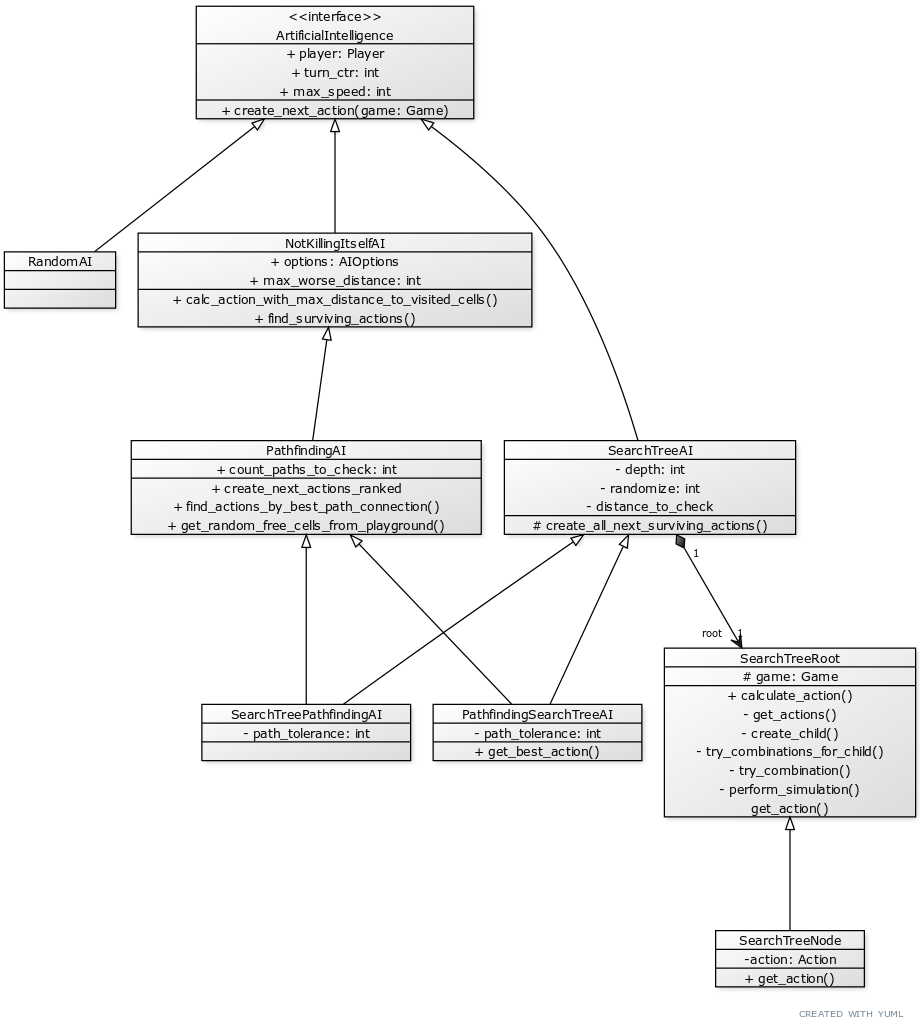
\includegraphics[width=0.8\textwidth]{Bilder/Klassendiagramm_AIs.png}
	\caption{UML-Klassendiagramm der \ac{KI}s}
	\label{fig:klassendiagramm-AIs}
\end{figure}

\section{Implementierung}
\label{sec:anhang-implementierung}

\begin{figure}[htb]
	\centering
	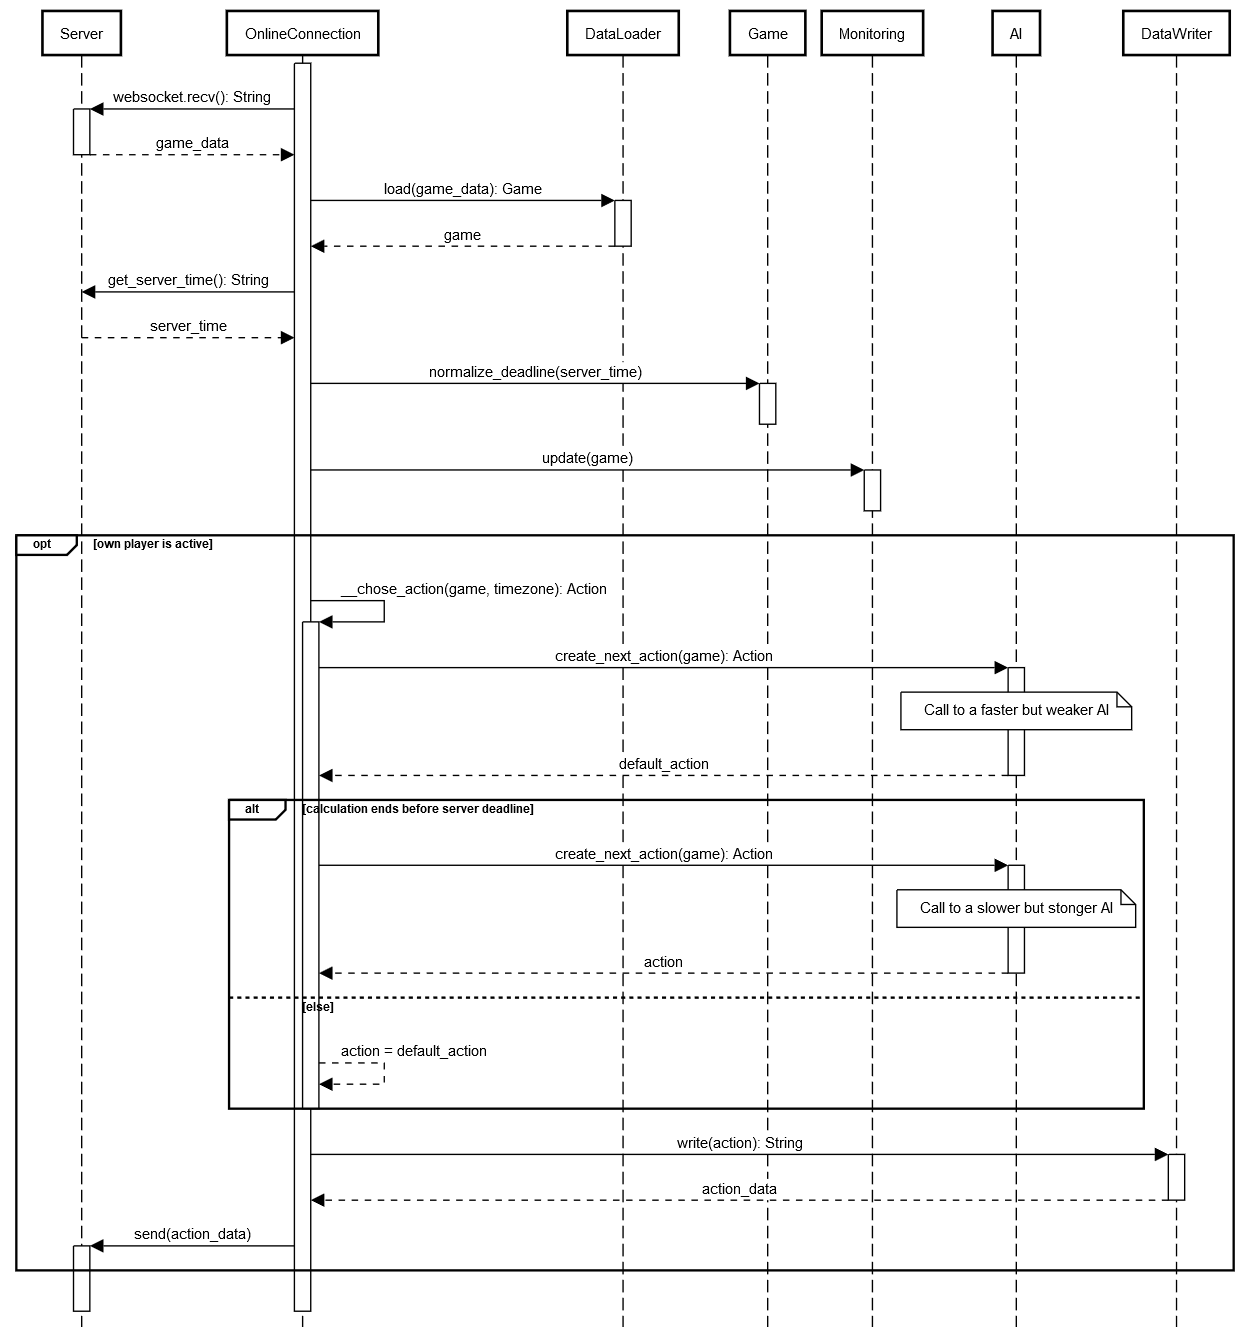
\includegraphics[width=\textwidth]{Bilder/Sequenzdiagramm_Implementierung_Spielzug.png}
	\caption{Sequenzdiagramm zur Implementierung eines Spielzug}
	\label{fig:sequenzdiagramm-spielzug}
\end{figure}

\begin{minipage}{\textwidth}
	\lstinputlisting[label=lst:online-__play,language=Python,caption=\Code{\_\_play()}-Methode des \Code{OnlineController}s]
	{./Dokumente/OnlineController-__play.txt}
\end{minipage}

\begin{minipage}{\textwidth}
	\lstinputlisting[label=lst:json-spiel,language=JSON,caption=JSON-Repräsentation eines Spiel-Zustands]
	{../tests/test_data/ai/game_2.json}
\end{minipage}

\begin{figure}[htb]
	\centering
	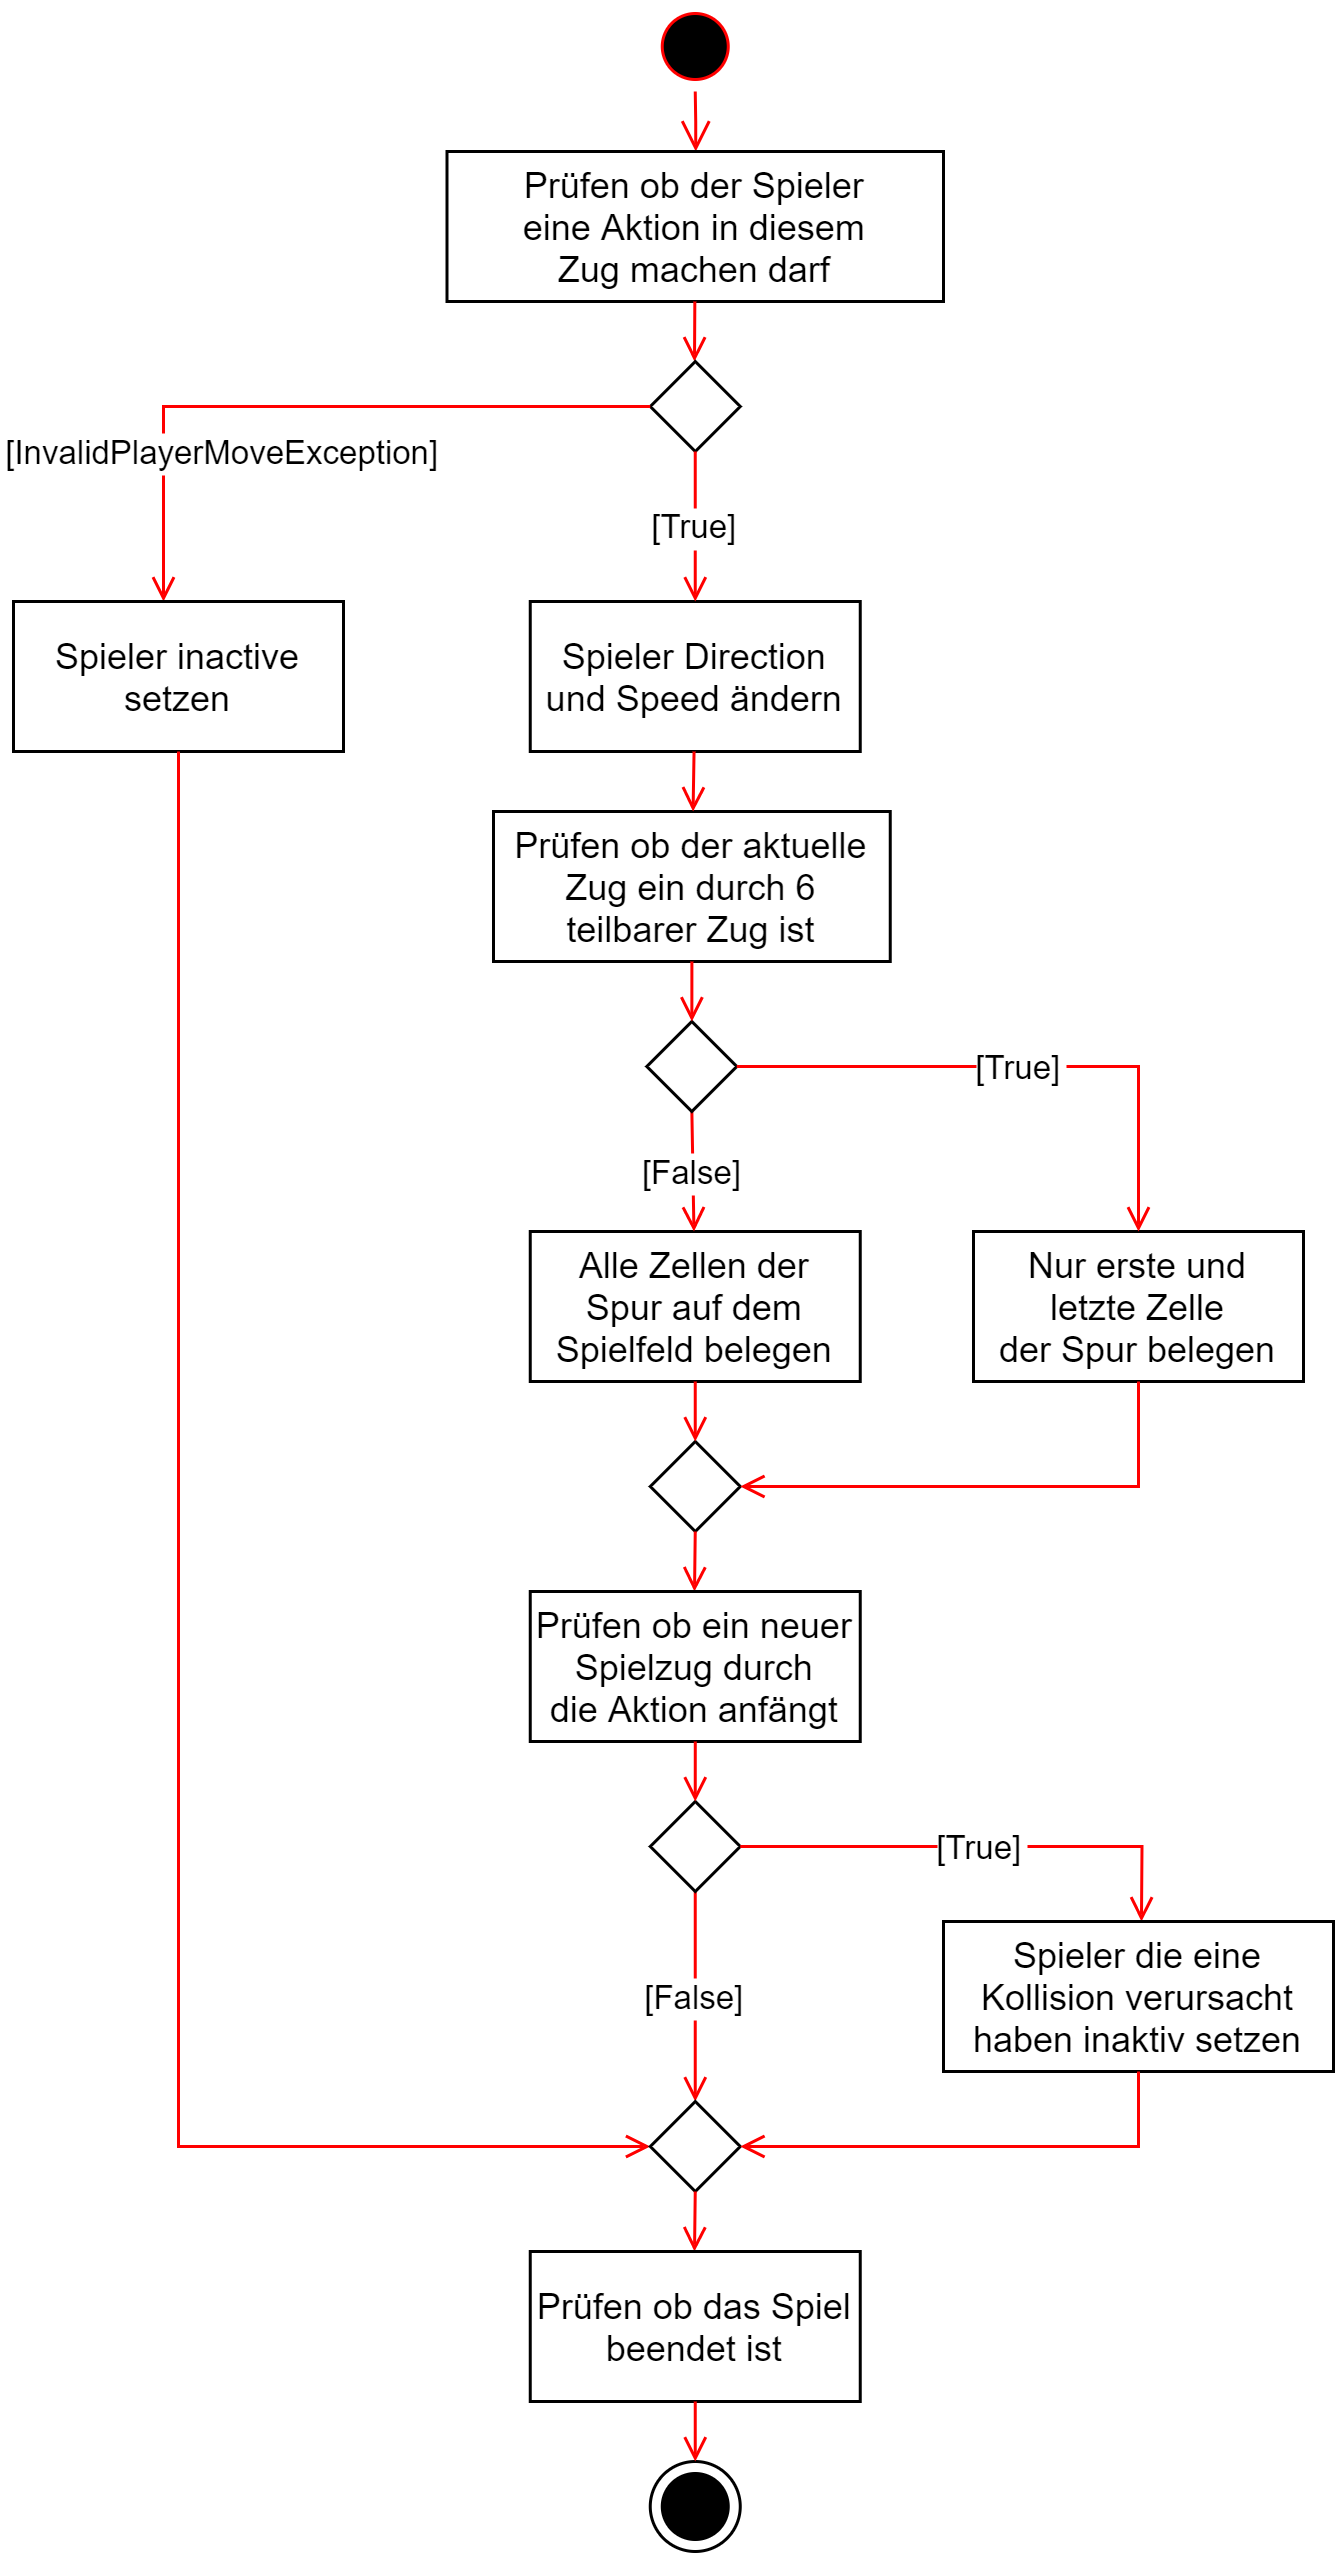
\includegraphics[width=0.7\textwidth]{Bilder/game_service_do_action_activity_diagram.png}
	\caption{Aktivitätsdiagramm zur Durchführung einer Spieler-Aktion durch den \Code{GameService}}
	\label{fig:aktivitaetsdiagramm-spieleraktion-gameservice}
\end{figure}

\begin{minipage}{\textwidth}
	\lstinputlisting[label=lst:get-and-visit-cells
	,language=Python,caption=\Code{get\_and\_visit\_cells(player, action)}-Methode des \Code{GameService}]
	{./Dokumente/Get_And_Visit_Cells_GameService.txt}
\end{minipage}

\begin{minipage}{\textwidth}
	\lstinputlisting[label=lst:pygame_update
	,language=Python,caption=\Code{update(game: Game)}-Methode der \Code{GraphicalView}]
	{./Dokumente/graphicalview_update.txt}
\end{minipage}

\section{Evaluation des besten Lösungsansatzes}
\label{sec:anhang-evaluation-loesungsansatz}

\begin{figure}[htb]
	\centering
	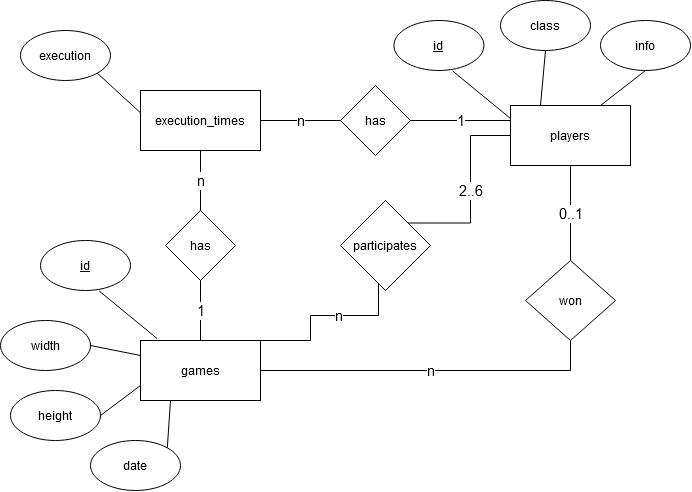
\includegraphics[width=0.8\textwidth]{Bilder/er-diagram.png}
	\caption{Entity-Relationship-Modell der Evaluations-Datenbank}
	\label{fig:er-schema}
\end{figure}

\begin{figure}[htb]
	\centering
	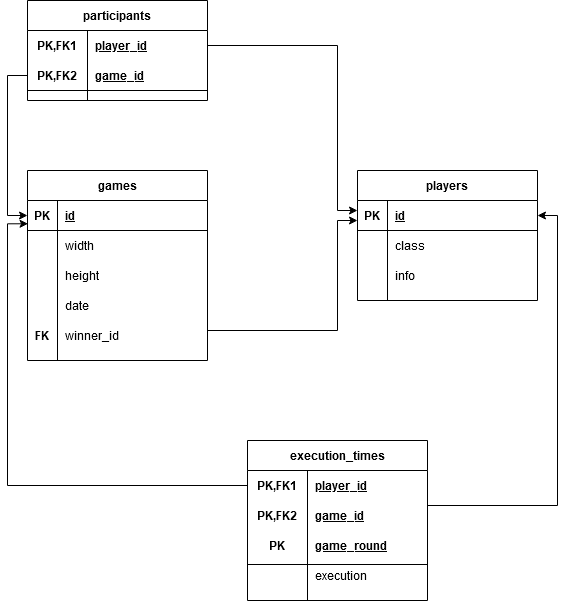
\includegraphics[width=0.8\textwidth]{Bilder/relationales_db_schema.png}
	\caption{Relationales Datenbankschema der Evaluations-Datenbank}
	\label{fig:relationales-db-schema}
\end{figure}

\section{Weiterentwicklung}
\label{sec:anhang-weiterentwicklung}

\begin{minipage}{\textwidth}
	\lstinputlisting[label=lst:yaml-github-action,language=YAML,caption=YAML-Konfiguration der Github Action]
	{../.github/workflows/python-app.yml}
\end{minipage}



%%%%%%%%%%%%%%%%%%%%%%%%%%%%%%%%%%%%%%%%%%%%%%%
%%%%%%%%% Literaturverzeichnis %%%%%%%%%%%%%%%%
%%%%%%%%%%%%%%%%%%%%%%%%%%%%%%%%%%%%%%%%%%%%%%%

\pagebreak
\addcontentsline{toc}{chapter}{Literaturverzeichnis}
\bibliographystyle{ieeetr}
\bibliography{literatur}

\end{document}
